%%%%%%%%%%%%%%%%%%%%%%%%%%%%%%%%%%%%%%%%%
% Beamer Presentation LaTeX Template Version 1.0 (10/11/12)
%
% This template has been downloaded from:
% http://www.LaTeXTemplates.com
%
% License: CC BY-NC-SA 3.0
% (http://creativecommons.org/licenses/by-nc-sa/3.0/)
%
%%%%%%%%%%%%%%%%%%%%%%%%%%%%%%%%%%%%%%%%%

% ----------------------------------------------------------------------------------------
% PACKAGES AND THEMES
% ----------------------------------------------------------------------------------------

\documentclass{beamer}

\mode<presentation> {

  % The Beamer class comes with a number of default slide themes which
  % change the colors and layouts of slides. Below this is a list of
  % all the themes, uncomment each in turn to see what they look like.

  % \usetheme{default} \usetheme{AnnArbor} \usetheme{Antibes}
  % \usetheme{Bergen} \usetheme{Berkeley} \usetheme{Berlin}
  % \usetheme{Boadilla} \usetheme{CambridgeUS} \usetheme{Copenhagen}
  % \usetheme{Darmstadt} \usetheme{Dresden} \usetheme{Frankfurt}
  % \usetheme{Goettingen} \usetheme{Hannover} \usetheme{Ilmenau}
  % \usetheme{JuanLesPins} \usetheme{Luebeck}
  \usetheme{Madrid}
  % \usetheme{Malmoe} \usetheme{Marburg} \usetheme{Montpellier}
  % \usetheme{PaloAlto} \usetheme{Pittsburgh} \usetheme{Rochester}
  % \usetheme{Singapore} \usetheme{Szeged} \usetheme{Warsaw}

  % As well as themes, the Beamer class has a number of color themes
  % for any slide theme. Uncomment each of these in turn to see how it
  % changes the colors of your current slide theme.

  % \usecolortheme{albatross}
  \usecolortheme{beaver}
  % \usecolortheme{beetle} \usecolortheme{crane}
  % \usecolortheme{dolphin} \usecolortheme{dove} \usecolortheme{fly}
  % \usecolortheme{lily} \usecolortheme{orchid} \usecolortheme{rose}
  % \usecolortheme{seagull} \usecolortheme{seahorse}
  % \usecolortheme{whale} \usecolortheme{wolverine}

  % \setbeamertemplate{footline} % To remove the footer line in all slides uncomment this line
  % \setbeamertemplate{footline}[page
  % number] % To replace the footer line in all slides with a simple slide count uncomment this line

  % \setbeamertemplate{navigation
  % symbols}{} % To remove the navigation symbols from the bottom of all slides uncomment this line
}
% xtong's tools
% aliasis
\newcommand{\xemp}[1]{{\color{red}{\textbf{#1}}}}
\newcommand{\bs}{\boldsymbol}
\newcommand{\mean}[2]{\left\langle{#1}\right\rangle_{#2}}
\newcommand{\trb}[1]{\textrm{Tr}\left({#1}\right)}
\newcommand{\trs}[1]{\textrm{Tr}\left[{#1}\right]}
\newcommand{\invb}[1]{{\left({#1}\right)^-}}
\newcommand{\invs}[1]{{\left[{#1}\right]^-}}
\newcommand\numberthis{\addtocounter{equation}{1}\tag{\theequation}}
\renewcommand{\eqref}[1]{Eq.\,\ref{#1}}
%
% vectors and matrices
\newcommand{\va}{\mathbf{a}}
\newcommand{\vb}{\mathbf{b}}
\newcommand{\vc}{\mathbf{c}}
\newcommand{\vf}{\mathbf{f}}
\newcommand{\vg}{\mathbf{g}}
\newcommand{\vh}{\mathbf{h}}
\newcommand{\vv}{\mathbf{v}}
\newcommand{\vx}{\mathbf{x}}
\newcommand{\vu}{\mathbf{u}}
\newcommand{\vy}{\mathbf{y}}
\newcommand{\vw}{\mathbf{w}}
\newcommand{\vs}{\mathbf{s}}
% 
\newcommand{\xf}{\mathbf{F}}
\newcommand{\xg}{\mathbf{G}}
\newcommand{\xh}{\mathbf{H}}
\newcommand{\xk}{\mathbf{K}}
\newcommand{\xl}{\mathbf{L}}
\newcommand{\xr}{\mathbf{R}}
%
\newcommand{\xu}{\mathbf{U}}
\newcommand{\xv}{\mathbf{V}}
\newcommand{\xx}{\mathbf{X}}
\newcommand{\xw}{\mathbf{W}}
\newcommand{\xy}{\mathbf{Y}}
\newcommand{\xz}{\mathbf{Z}}
\newcommand{\xa}{\mathbf{A}}
\newcommand{\xd}{\mathbf{D}}
% 
% with tildes
%% vectors
\newcommand{\vat}{\tilde{\vb}}
\newcommand{\vbt}{\tilde{\vb}}
\newcommand{\vct}{\tilde{\vc}}
\newcommand{\vht}{\tilde{\vh}}
\newcommand{\vvt}{\tilde{\vv}}
\newcommand{\vst}{\tilde{\vs}}
\newcommand{\vut}{\tilde{\vu}}
\newcommand{\vft}{\tilde{\vf}}
\newcommand{\xut}{\tilde{\xu}}
\newcommand{\vxt}{\tilde{\vx}}
\newcommand{\xvt}{\tilde{\xv}}
\newcommand{\xyt}{\tilde{\xy}}
%% matrices
\newcommand{\xwt}{\tilde{\xw}}
%
% with hats
\newcommand{\vhh}{\hat{\vh}}
\newcommand{\xvh}{\hat{\xv}}
\newcommand{\vvh}{\hat{\vv}}
\newcommand{\vyh}{\hat{\vy}}
\newcommand{\vxh}{\hat{\vx}}
\newcommand{\vuh}{\hat{\vu}}
\newcommand{\vfh}{\hat{\vf}}
\newcommand{\xyh}{\hat{\xy}}
\newcommand{\xxh}{\hat{\xx}}
\newcommand{\xuh}{\hat{\xu}}
%
%
% derivatives
\newcommand{\DRV}[2]{\frac{d #1}{d #2}}
\newcommand{\DRC}[3]{\DRV{#1}{#2}\DRV{#2}{#3}}
\newcommand{\PDV}[2]{\frac{\partial #1}{\partial #2}}
\newcommand{\PDC}[3]{\PDV{#1}{#2}\PDV{#2}{#3}}
%
% the diagnal matrix
\newcommand{\id}{\textrm{\textbf{I}}}
\newcommand{\im}{\textrm{\textbf{I}}}
% the vector of ones
\newcommand{\one}{\mathbf{1}}
% 
% xiaoran's edit
\newcommand{\xadd}[1]{\textcolor{blue}{#1}}
\newcommand{\xdel}[1]{\textcolor{red}{\sout{#1}}}
\newcommand{\xrpl}[2]{\xdel{#1}\xadd{#2}}
\newcommand{\xacc}[1]{\textcolor{ForestGreen}{#1}}
%
%
% declarations
% argument of the minimum / maximum
\DeclareMathOperator*{\argmin}{arg\,min}
\DeclareMathOperator*{\argmax}{arg\,max}
%
% norms
\newcommand\norm[1]{\left\lVert#1\right\rVert}
%%%%% NEW MATH DEFINITIONS %%%%%

% Mark sections of captions for referring to divisions of figures
\newcommand{\figleft}{{\em (Left)}}
\newcommand{\figcenter}{{\em (Center)}}
\newcommand{\figright}{{\em (Right)}}
\newcommand{\figtop}{{\em (Top)}}
\newcommand{\figbottom}{{\em (Bottom)}}
\newcommand{\captiona}{{\em (a)}}
\newcommand{\captionb}{{\em (b)}}
\newcommand{\captionc}{{\em (c)}}
\newcommand{\captiond}{{\em (d)}}

% Highlight a newly defined term
\newcommand{\newterm}[1]{{\bf #1}}


% Figure reference, lower-case.
\def\figref#1{figure~\ref{#1}}
% Figure reference, capital. For start of sentence
\def\Figref#1{Figure~\ref{#1}}
\def\twofigref#1#2{figures \ref{#1} and \ref{#2}}
\def\quadfigref#1#2#3#4{figures \ref{#1}, \ref{#2}, \ref{#3} and \ref{#4}}
% Section reference, lower-case.
\def\secref#1{section~\ref{#1}}
% Section reference, capital.
\def\Secref#1{Section~\ref{#1}}
% Reference to two sections.
\def\twosecrefs#1#2{sections \ref{#1} and \ref{#2}}
% Reference to three sections.
\def\secrefs#1#2#3{sections \ref{#1}, \ref{#2} and \ref{#3}}
% Reference to an equation, lower-case.
\def\eqref#1{equation~\ref{#1}}
% Reference to an equation, upper case
\def\Eqref#1{Equation~\ref{#1}}
% A raw reference to an equation---avoid using if possible
\def\plaineqref#1{\ref{#1}}
% Reference to a chapter, lower-case.
\def\chapref#1{chapter~\ref{#1}}
% Reference to an equation, upper case.
\def\Chapref#1{Chapter~\ref{#1}}
% Reference to a range of chapters
\def\rangechapref#1#2{chapters\ref{#1}--\ref{#2}}
% Reference to an algorithm, lower-case.
\def\algref#1{algorithm~\ref{#1}}
% Reference to an algorithm, upper case.
\def\Algref#1{Algorithm~\ref{#1}}
\def\twoalgref#1#2{algorithms \ref{#1} and \ref{#2}}
\def\Twoalgref#1#2{Algorithms \ref{#1} and \ref{#2}}
% Reference to a part, lower case
\def\partref#1{part~\ref{#1}}
% Reference to a part, upper case
\def\Partref#1{Part~\ref{#1}}
\def\twopartref#1#2{parts \ref{#1} and \ref{#2}}

\def\ceil#1{\lceil #1 \rceil}
\def\floor#1{\lfloor #1 \rfloor}
\def\1{\bm{1}}
\newcommand{\train}{\mathcal{D}}
\newcommand{\valid}{\mathcal{D_{\mathrm{valid}}}}
\newcommand{\test}{\mathcal{D_{\mathrm{test}}}}

\def\eps{{\epsilon}}


% Random variables
\def\reta{{\textnormal{$\eta$}}}
\def\ra{{\textnormal{a}}}
\def\rb{{\textnormal{b}}}
\def\rc{{\textnormal{c}}}
\def\rd{{\textnormal{d}}}
\def\re{{\textnormal{e}}}
\def\rf{{\textnormal{f}}}
\def\rg{{\textnormal{g}}}
\def\rh{{\textnormal{h}}}
\def\ri{{\textnormal{i}}}
\def\rj{{\textnormal{j}}}
\def\rk{{\textnormal{k}}}
\def\rl{{\textnormal{l}}}
% rm is already a command, just don't name any random variables m
\def\rn{{\textnormal{n}}}
\def\ro{{\textnormal{o}}}
\def\rp{{\textnormal{p}}}
\def\rq{{\textnormal{q}}}
\def\rr{{\textnormal{r}}}
\def\rs{{\textnormal{s}}}
\def\rt{{\textnormal{t}}}
\def\ru{{\textnormal{u}}}
\def\rv{{\textnormal{v}}}
\def\rw{{\textnormal{w}}}
\def\rx{{\textnormal{x}}}
\def\ry{{\textnormal{y}}}
\def\rz{{\textnormal{z}}}

% Random vectors
\def\rvepsilon{{\mathbf{\epsilon}}}
\def\rvtheta{{\mathbf{\theta}}}
\def\rva{{\mathbf{a}}}
\def\rvb{{\mathbf{b}}}
\def\rvc{{\mathbf{c}}}
\def\rvd{{\mathbf{d}}}
\def\rve{{\mathbf{e}}}
\def\rvf{{\mathbf{f}}}
\def\rvg{{\mathbf{g}}}
\def\rvh{{\mathbf{h}}}
\def\rvu{{\mathbf{i}}}
\def\rvj{{\mathbf{j}}}
\def\rvk{{\mathbf{k}}}
\def\rvl{{\mathbf{l}}}
\def\rvm{{\mathbf{m}}}
\def\rvn{{\mathbf{n}}}
\def\rvo{{\mathbf{o}}}
\def\rvp{{\mathbf{p}}}
\def\rvq{{\mathbf{q}}}
\def\rvr{{\mathbf{r}}}
\def\rvs{{\mathbf{s}}}
\def\rvt{{\mathbf{t}}}
\def\rvu{{\mathbf{u}}}
\def\rvv{{\mathbf{v}}}
\def\rvw{{\mathbf{w}}}
\def\rvx{{\mathbf{x}}}
\def\rvy{{\mathbf{y}}}
\def\rvz{{\mathbf{z}}}

% Elements of random vectors
\def\erva{{\textnormal{a}}}
\def\ervb{{\textnormal{b}}}
\def\ervc{{\textnormal{c}}}
\def\ervd{{\textnormal{d}}}
\def\erve{{\textnormal{e}}}
\def\ervf{{\textnormal{f}}}
\def\ervg{{\textnormal{g}}}
\def\ervh{{\textnormal{h}}}
\def\ervi{{\textnormal{i}}}
\def\ervj{{\textnormal{j}}}
\def\ervk{{\textnormal{k}}}
\def\ervl{{\textnormal{l}}}
\def\ervm{{\textnormal{m}}}
\def\ervn{{\textnormal{n}}}
\def\ervo{{\textnormal{o}}}
\def\ervp{{\textnormal{p}}}
\def\ervq{{\textnormal{q}}}
\def\ervr{{\textnormal{r}}}
\def\ervs{{\textnormal{s}}}
\def\ervt{{\textnormal{t}}}
\def\ervu{{\textnormal{u}}}
\def\ervv{{\textnormal{v}}}
\def\ervw{{\textnormal{w}}}
\def\ervx{{\textnormal{x}}}
\def\ervy{{\textnormal{y}}}
\def\ervz{{\textnormal{z}}}

% Random matrices
\def\rmA{{\mathbf{A}}}
\def\rmB{{\mathbf{B}}}
\def\rmC{{\mathbf{C}}}
\def\rmD{{\mathbf{D}}}
\def\rmE{{\mathbf{E}}}
\def\rmF{{\mathbf{F}}}
\def\rmG{{\mathbf{G}}}
\def\rmH{{\mathbf{H}}}
\def\rmI{{\mathbf{I}}}
\def\rmJ{{\mathbf{J}}}
\def\rmK{{\mathbf{K}}}
\def\rmL{{\mathbf{L}}}
\def\rmM{{\mathbf{M}}}
\def\rmN{{\mathbf{N}}}
\def\rmO{{\mathbf{O}}}
\def\rmP{{\mathbf{P}}}
\def\rmQ{{\mathbf{Q}}}
\def\rmR{{\mathbf{R}}}
\def\rmS{{\mathbf{S}}}
\def\rmT{{\mathbf{T}}}
\def\rmU{{\mathbf{U}}}
\def\rmV{{\mathbf{V}}}
\def\rmW{{\mathbf{W}}}
\def\rmX{{\mathbf{X}}}
\def\rmY{{\mathbf{Y}}}
\def\rmZ{{\mathbf{Z}}}

% Elements of random matrices
\def\ermA{{\textnormal{A}}}
\def\ermB{{\textnormal{B}}}
\def\ermC{{\textnormal{C}}}
\def\ermD{{\textnormal{D}}}
\def\ermE{{\textnormal{E}}}
\def\ermF{{\textnormal{F}}}
\def\ermG{{\textnormal{G}}}
\def\ermH{{\textnormal{H}}}
\def\ermI{{\textnormal{I}}}
\def\ermJ{{\textnormal{J}}}
\def\ermK{{\textnormal{K}}}
\def\ermL{{\textnormal{L}}}
\def\ermM{{\textnormal{M}}}
\def\ermN{{\textnormal{N}}}
\def\ermO{{\textnormal{O}}}
\def\ermP{{\textnormal{P}}}
\def\ermQ{{\textnormal{Q}}}
\def\ermR{{\textnormal{R}}}
\def\ermS{{\textnormal{S}}}
\def\ermT{{\textnormal{T}}}
\def\ermU{{\textnormal{U}}}
\def\ermV{{\textnormal{V}}}
\def\ermW{{\textnormal{W}}}
\def\ermX{{\textnormal{X}}}
\def\ermY{{\textnormal{Y}}}
\def\ermZ{{\textnormal{Z}}}

% Vectors
\def\vzero{{\bm{0}}}
\def\vone{{\bm{1}}}
\def\vmu{{\bm{\mu}}}
\def\vtheta{{\bm{\theta}}}
\def\va{{\bm{a}}}
\def\vb{{\bm{b}}}
\def\vc{{\bm{c}}}
\def\vd{{\bm{d}}}
\def\ve{{\bm{e}}}
\def\vf{{\bm{f}}}
\def\vg{{\bm{g}}}
\def\vh{{\bm{h}}}
\def\vi{{\bm{i}}}
\def\vj{{\bm{j}}}
\def\vk{{\bm{k}}}
\def\vl{{\bm{l}}}
\def\vm{{\bm{m}}}
\def\vn{{\bm{n}}}
\def\vo{{\bm{o}}}
\def\vp{{\bm{p}}}
\def\vq{{\bm{q}}}
\def\vr{{\bm{r}}}
\def\vs{{\bm{s}}}
\def\vt{{\bm{t}}}
\def\vu{{\bm{u}}}
\def\vv{{\bm{v}}}
\def\vw{{\bm{w}}}
\def\vx{{\bm{x}}}
\def\vy{{\bm{y}}}
\def\vz{{\bm{z}}}

% Elements of vectors
\def\evalpha{{\alpha}}
\def\evbeta{{\beta}}
\def\evepsilon{{\epsilon}}
\def\evlambda{{\lambda}}
\def\evomega{{\omega}}
\def\evmu{{\mu}}
\def\evpsi{{\psi}}
\def\evsigma{{\sigma}}
\def\evtheta{{\theta}}
\def\eva{{a}}
\def\evb{{b}}
\def\evc{{c}}
\def\evd{{d}}
\def\eve{{e}}
\def\evf{{f}}
\def\evg{{g}}
\def\evh{{h}}
\def\evi{{i}}
\def\evj{{j}}
\def\evk{{k}}
\def\evl{{l}}
\def\evm{{m}}
\def\evn{{n}}
\def\evo{{o}}
\def\evp{{p}}
\def\evq{{q}}
\def\evr{{r}}
\def\evs{{s}}
\def\evt{{t}}
\def\evu{{u}}
\def\evv{{v}}
\def\evw{{w}}
\def\evx{{x}}
\def\evy{{y}}
\def\evz{{z}}

% Matrix
\def\mA{{\bm{A}}}
\def\mB{{\bm{B}}}
\def\mC{{\bm{C}}}
\def\mD{{\bm{D}}}
\def\mE{{\bm{E}}}
\def\mF{{\bm{F}}}
\def\mG{{\bm{G}}}
\def\mH{{\bm{H}}}
\def\mI{{\bm{I}}}
\def\mJ{{\bm{J}}}
\def\mK{{\bm{K}}}
\def\mL{{\bm{L}}}
\def\mM{{\bm{M}}}
\def\mN{{\bm{N}}}
\def\mO{{\bm{O}}}
\def\mP{{\bm{P}}}
\def\mQ{{\bm{Q}}}
\def\mR{{\bm{R}}}
\def\mS{{\bm{S}}}
\def\mT{{\bm{T}}}
\def\mU{{\bm{U}}}
\def\mV{{\bm{V}}}
\def\mW{{\bm{W}}}
\def\mX{{\bm{X}}}
\def\mY{{\bm{Y}}}
\def\mZ{{\bm{Z}}}
\def\mBeta{{\bm{\beta}}}
\def\mPhi{{\bm{\Phi}}}
\def\mLambda{{\bm{\Lambda}}}
\def\mSigma{{\bm{\Sigma}}}

% Tensor
\DeclareMathAlphabet{\mathsfit}{\encodingdefault}{\sfdefault}{m}{sl}
\SetMathAlphabet{\mathsfit}{bold}{\encodingdefault}{\sfdefault}{bx}{n}
\newcommand{\tens}[1]{\bm{\mathsfit{#1}}}
\def\tA{{\tens{A}}}
\def\tB{{\tens{B}}}
\def\tC{{\tens{C}}}
\def\tD{{\tens{D}}}
\def\tE{{\tens{E}}}
\def\tF{{\tens{F}}}
\def\tG{{\tens{G}}}
\def\tH{{\tens{H}}}
\def\tI{{\tens{I}}}
\def\tJ{{\tens{J}}}
\def\tK{{\tens{K}}}
\def\tL{{\tens{L}}}
\def\tM{{\tens{M}}}
\def\tN{{\tens{N}}}
\def\tO{{\tens{O}}}
\def\tP{{\tens{P}}}
\def\tQ{{\tens{Q}}}
\def\tR{{\tens{R}}}
\def\tS{{\tens{S}}}
\def\tT{{\tens{T}}}
\def\tU{{\tens{U}}}
\def\tV{{\tens{V}}}
\def\tW{{\tens{W}}}
\def\tX{{\tens{X}}}
\def\tY{{\tens{Y}}}
\def\tZ{{\tens{Z}}}


% Graph
\def\gA{{\mathcal{A}}}
\def\gB{{\mathcal{B}}}
\def\gC{{\mathcal{C}}}
\def\gD{{\mathcal{D}}}
\def\gE{{\mathcal{E}}}
\def\gF{{\mathcal{F}}}
\def\gG{{\mathcal{G}}}
\def\gH{{\mathcal{H}}}
\def\gI{{\mathcal{I}}}
\def\gJ{{\mathcal{J}}}
\def\gK{{\mathcal{K}}}
\def\gL{{\mathcal{L}}}
\def\gM{{\mathcal{M}}}
\def\gN{{\mathcal{N}}}
\def\gO{{\mathcal{O}}}
\def\gP{{\mathcal{P}}}
\def\gQ{{\mathcal{Q}}}
\def\gR{{\mathcal{R}}}
\def\gS{{\mathcal{S}}}
\def\gT{{\mathcal{T}}}
\def\gU{{\mathcal{U}}}
\def\gV{{\mathcal{V}}}
\def\gW{{\mathcal{W}}}
\def\gX{{\mathcal{X}}}
\def\gY{{\mathcal{Y}}}
\def\gZ{{\mathcal{Z}}}

% Sets
\def\sA{{\mathbb{A}}}
\def\sB{{\mathbb{B}}}
\def\sC{{\mathbb{C}}}
\def\sD{{\mathbb{D}}}
% Don't use a set called E, because this would be the same as our symbol
% for expectation.
\def\sF{{\mathbb{F}}}
\def\sG{{\mathbb{G}}}
\def\sH{{\mathbb{H}}}
\def\sI{{\mathbb{I}}}
\def\sJ{{\mathbb{J}}}
\def\sK{{\mathbb{K}}}
\def\sL{{\mathbb{L}}}
\def\sM{{\mathbb{M}}}
\def\sN{{\mathbb{N}}}
\def\sO{{\mathbb{O}}}
\def\sP{{\mathbb{P}}}
\def\sQ{{\mathbb{Q}}}
\def\sR{{\mathbb{R}}}
\def\sS{{\mathbb{S}}}
\def\sT{{\mathbb{T}}}
\def\sU{{\mathbb{U}}}
\def\sV{{\mathbb{V}}}
\def\sW{{\mathbb{W}}}
\def\sX{{\mathbb{X}}}
\def\sY{{\mathbb{Y}}}
\def\sZ{{\mathbb{Z}}}

% Entries of a matrix
\def\emLambda{{\Lambda}}
\def\emA{{A}}
\def\emB{{B}}
\def\emC{{C}}
\def\emD{{D}}
\def\emE{{E}}
\def\emF{{F}}
\def\emG{{G}}
\def\emH{{H}}
\def\emI{{I}}
\def\emJ{{J}}
\def\emK{{K}}
\def\emL{{L}}
\def\emM{{M}}
\def\emN{{N}}
\def\emO{{O}}
\def\emP{{P}}
\def\emQ{{Q}}
\def\emR{{R}}
\def\emS{{S}}
\def\emT{{T}}
\def\emU{{U}}
\def\emV{{V}}
\def\emW{{W}}
\def\emX{{X}}
\def\emY{{Y}}
\def\emZ{{Z}}
\def\emSigma{{\Sigma}}

% entries of a tensor
% Same font as tensor, without \bm wrapper
\newcommand{\etens}[1]{\mathsfit{#1}}
\def\etLambda{{\etens{\Lambda}}}
\def\etA{{\etens{A}}}
\def\etB{{\etens{B}}}
\def\etC{{\etens{C}}}
\def\etD{{\etens{D}}}
\def\etE{{\etens{E}}}
\def\etF{{\etens{F}}}
\def\etG{{\etens{G}}}
\def\etH{{\etens{H}}}
\def\etI{{\etens{I}}}
\def\etJ{{\etens{J}}}
\def\etK{{\etens{K}}}
\def\etL{{\etens{L}}}
\def\etM{{\etens{M}}}
\def\etN{{\etens{N}}}
\def\etO{{\etens{O}}}
\def\etP{{\etens{P}}}
\def\etQ{{\etens{Q}}}
\def\etR{{\etens{R}}}
\def\etS{{\etens{S}}}
\def\etT{{\etens{T}}}
\def\etU{{\etens{U}}}
\def\etV{{\etens{V}}}
\def\etW{{\etens{W}}}
\def\etX{{\etens{X}}}
\def\etY{{\etens{Y}}}
\def\etZ{{\etens{Z}}}

% The true underlying data generating distribution
\newcommand{\pdata}{p_{\rm{data}}}
% The empirical distribution defined by the training set
\newcommand{\ptrain}{\hat{p}_{\rm{data}}}
\newcommand{\Ptrain}{\hat{P}_{\rm{data}}}
% The model distribution
\newcommand{\pmodel}{p_{\rm{model}}}
\newcommand{\Pmodel}{P_{\rm{model}}}
\newcommand{\ptildemodel}{\tilde{p}_{\rm{model}}}
% Stochastic autoencoder distributions
\newcommand{\pencode}{p_{\rm{encoder}}}
\newcommand{\pdecode}{p_{\rm{decoder}}}
\newcommand{\precons}{p_{\rm{reconstruct}}}

\newcommand{\laplace}{\mathrm{Laplace}} % Laplace distribution

\newcommand{\E}{\mathbb{E}}
\newcommand{\Ls}{\mathcal{L}}
\newcommand{\R}{\mathbb{R}}
\newcommand{\emp}{\tilde{p}}
\newcommand{\lr}{\alpha}
\newcommand{\reg}{\lambda}
\newcommand{\rect}{\mathrm{rectifier}}
\newcommand{\softmax}{\mathrm{softmax}}
\newcommand{\sigmoid}{\sigma}
\newcommand{\softplus}{\zeta}
\newcommand{\KL}{D_{\mathrm{KL}}}
\newcommand{\Var}{\mathrm{Var}}
\newcommand{\standarderror}{\mathrm{SE}}
\newcommand{\Cov}{\mathrm{Cov}}
% Wolfram Mathworld says $L^2$ is for function spaces and $\ell^2$ is for vectors
% But then they seem to use $L^2$ for vectors throughout the site, and so does
% wikipedia.
\newcommand{\normlzero}{L^0}
\newcommand{\normlone}{L^1}
\newcommand{\normltwo}{L^2}
\newcommand{\normlp}{L^p}
\newcommand{\normmax}{L^\infty}

\newcommand{\parents}{Pa} % See usage in notation.tex. Chosen to match Daphne's book.

\DeclareMathOperator*{\argmax}{arg\,max}
\DeclareMathOperator*{\argmin}{arg\,min}

\DeclareMathOperator{\sign}{sign}
\DeclareMathOperator{\Tr}{Tr}
\let\ab\allowbreak

\newcommand{\se}[1]{\hat{\mathtt{se}}\left(#1\right)} % standard error
\newcommand{\ti}{{\tilde{i}}} % tilde i
\newcommand{\ef}{{\mathtt{o}}} % error function
\newcommand{\kn}{\mathcal{K}} % kernel
\usepackage{graphicx} % Allows including images
\usepackage{booktabs} % Allows the use of \toprule, \midrule and \bottomrule in tables
\usepackage{bm}

% ----------------------------------------------------------------------------------------
% TITLE PAGE
% ----------------------------------------------------------------------------------------

\title[Fast-VCM]{Improved Variance Component Model \\ Simulation Studies}

\author{Xiaoran Tong} % Your name
\institute[EPI Biosta,
MSU] % Your institution as it will appear on the bottom of every slide, may be shorthand to save space
{ Michigan State University \\ % Your institution for the title page
  \medskip \textit{tongxia1@msu.edu} \\% Your email address
  \textit{qlu@epi.msu.edu} % Your email address
} \date{\today} % Date, can be changed to a custom date

\begin{document}

\begin{frame}
  \titlepage % Print the title page as the first slide
\end{frame}

\begin{frame}
  \frametitle{Table of
    Content} % Table of contents slide, comment this block out to remove it
  \tableofcontents
\end{frame}
% ----------------------------------------------------------------------------------------
% ----------------------------------------------------------------------------------------
% PRESENTATION SLIDES
% -------------------------------------------------------------------
\section{Motivation}
% -------------------------------------------------------------------
\begin{frame}\frametitle{Motivation: Issues}
  Analyzing ultra-high dimensional profiles are increasingly popular,
  e.g.,
  \begin{itemize}
  \item deeply sequenced genome
  \item neural imaginings (i.e., MRI, fMRI, DTI)
  \end{itemize}
  \textbf{Variance Component Model (VCM)} is a sensible choice to
  \begin{itemize}
  \item aggregate weak effect of massive number of correlated variants
  \item partially solve the curse of dimension: $N \times P \to N^2$
  \end{itemize}
  \textbf{VCM} is also known as
  \begin{itemize}
  \item kernel machine, kernel method
  \item random effect model
  \end{itemize}
\end{frame}
% -------------------------------------------------------------------
\newcommand{\fit}[1]{{\color{magenta}{#1}}}
\newcommand{\CB}[1]{{\color{blue}{#1}}}
\newcommand{\CR}[1]{{\color{red}{#1}}}
\newcommand{\green}[1]{{\color{green}{#1}}}
\begin{frame}
  \frametitle{Motivation: \CB{v}ariance \CB{c}omponent
    \CB{m}odel (\CB{\textbf{VCM}})} %
  \textbf{VCM} depicts the influence of ultra high dimensional $\xx$
  on $\vy$,
  \begin{align}\label{eq:vcm}
    h(\vy) = \vz \sim \mathcal{N}(0, \xv), \quad
    \xv = \fit{\sigma^2_0} \id + \fit{\sigma^2_1} \mck_1(\xx) + \dots + \fit{\sigma^2_L} \mck_L(\xx)
  \end{align}
  \begin{itemize}
  \item as the residual of $\vy$, $\vz$ follows MVN of covariance
    $\xv$;
  \item $\xv$ is the sum of $L$ kernels plus a white noise
    $\mck_0 = \id$;
  \item kernels are built from $\xx$
  \item The to be fitted
    $\vtheta = \{\fit{\sigma^2_0}, \fit{\sigma^2_1} \dots
    \fit{\sigma^2_L}\}$ comprises a \textbf{VCM}.
  \end{itemize}
\end{frame}
% -------------------------------------------------------------------
\begin{frame}
  \frametitle{Motivation: computation issues of \CB{\textbf{VCM}}} %
  \textbf{A VCM requires}
  \begin{itemize}
  \item multiple kernels ($L>1$) to achieve high capacity;
  \item large sample $N$ to stabilize;
  \item $O(N^3)$ to invert the combined kernel matrix.
  \end{itemize}
  \textbf{Re-introduce the curse of dimensionality by large cohorts.}
\end{frame}
% -------------------------------------------------------------------
\begin{frame}\frametitle{Motivation: \textbf{VCM:}} %
  \begin{figure}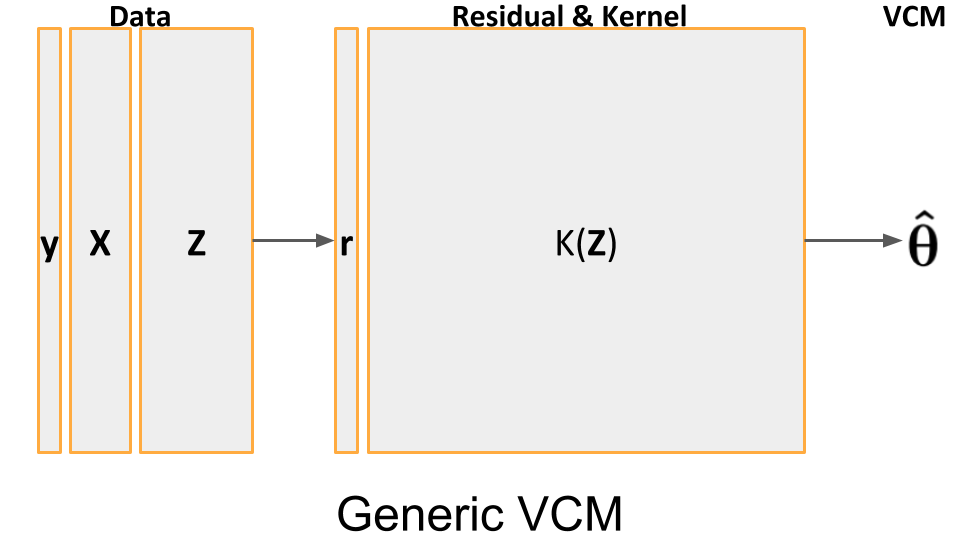
\includegraphics[width=1\textwidth]{img/vcm_org}\end{figure}
\end{frame}
% -------------------------------------------------------------------
\section{Improved VCM}
% -------------------------------------------------------------------
\begin{frame}
  \large{\textbf{Proposal}}: \\
  \large{\textbf{\CR{Batched, Deep, MINQUE} \CB{v}ariance \CB{c}omponent \CB{m}odel}} \\
  \textbf{Increase capacity}
  \begin{itemize}
  \item depen the kernels;
  \end{itemize}
  \textbf{Reduce computation}
  \begin{itemize}
  \item solve VCs in close form by MINQUE;
  \item built VCM by batch.
  \end{itemize}
\end{frame}
% -------------------------------------------------------------------
\begin{frame}%
  \frametitle{Deepen the Kernels}
  \textbf{``polynomial expansion'' by kernel:}
  \begin{align*}
    \xk^{(1)} & = \bigcup_{i}^L \kn_i(\xx) = \{\xk_1, \dots, \xk_L\} \\
    \xk^{(2)} & = \bigcup_{i,j}^{L \times L} \kn_i(\xx) \circ \kn_j(\xx) = \{\xk_1\xk_1, \xk_1\xk_2, \dots, \xk_L\xk_L\} \\
    \xk^{(3)} & = \bigcup_{i,j,k}^{L^{(3)}}  \kn_i(\xx) \circ \kn_j(\xx) \circ \kn_k(\xx)
  \end{align*}
  \CB{\textbf{improve model capacity.}}
\end{frame}
% -------------------------------------------------------------------
\begin{frame} %
  \frametitle{MINQUE} %
  \textbf{use \CB{MINQUE} for estimation}
  \begin{itemize}
  \item faster by solving $\vtheta=\{\sigma_0^2, \sigma_1^2, \dots \}$
    in close form;
  \item numerically more stable via generalized inverse;
  \item no assumption on $\vz$'s distribution.
  \end{itemize}
  MINQUE -- minimum norm quadratic unbiased estimation, developed
  by (\textbf{Rao et. al.}, 1971).
\end{frame}
% -------------------------------------------------------------------
\begin{frame}\frametitle{Batched Training}
  \begin{enumerate}
  \item randomly partition the cohort into Q batches $b_i = (\vy_i, \mM_i, \mX_i)$;
  \item for $i = 1 \dots Q$:
    \begin{itemize}
    \item calculate $(\vr_i, \tK_i) = (h(\vy_i), \mathcal{K}_{1 \dots L}(\mX_i))$
    \item solve the $i$ th. VCM, $\vtheta_i^{(j)}$
    \end{itemize}
  \item repeat \textbf{1} and \textbf{2} for $j=1 \dots R$ epochs
  \item let $\hat{\vtheta} = \frac
    {\sum_{i=1}^Q\sum_{j=1}^R w_i^{(j)}\vtheta_i^{(j)}}
    {\sum_{\tilde{i}=1}^Q \sum_{\tilde{j}=1}^R w_{\tilde{i}}^{(\tilde{j})}}$
  \end{enumerate}
  When the sample size $N$ is huge, and the batch size $\frac{N}{Q}$ large enough to
  stabilize each VCM, a single run-through ($R=1$) is sufficient.
\end{frame}
% -------------------------------------------------------------------
\begin{frame}\frametitle{Whole Sample VCM versus Batched VCM:} %
  \begin{figure}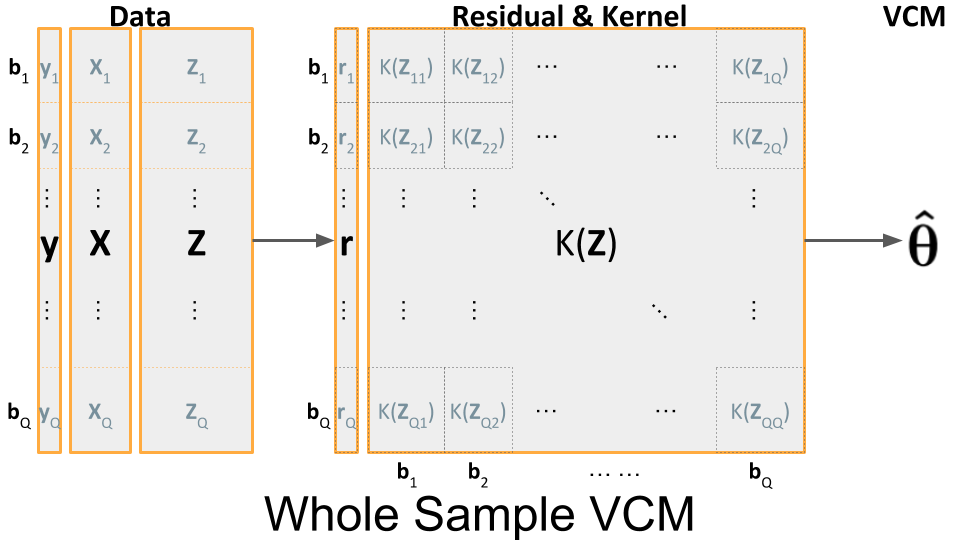
\includegraphics[width=1\textwidth]{img/vcm_whl}\end{figure}
\end{frame}
\begin{frame}\frametitle{Whole Sample VCM versus Batched VCM:} %
  \begin{figure}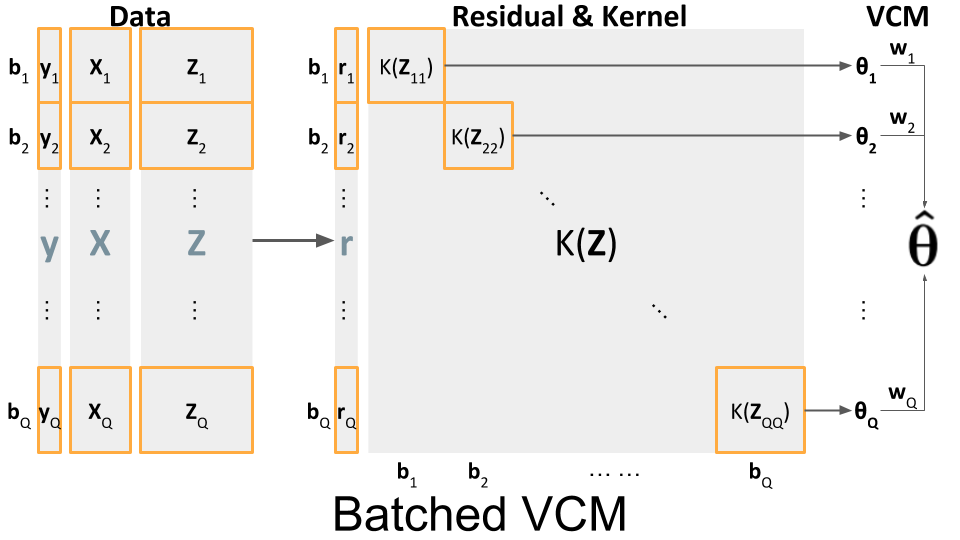
\includegraphics[width=1\textwidth]{img/vcm_bat}\end{figure}
\end{frame}
% -------------------------------------------------------------------
\section{Simulation}
\begin{frame}
  \frametitle{Simulation: Scenarios} %
  \centering
  \Large{\textbf{Simulation Studies}}
  \normalsize
  \begin{itemize}
  \item performance of improved VCM versus GCTA-REML;
  \item performance batched training VCM versus whole sample training;
  \item running time.
  \end{itemize}
\end{frame}
% -------------------------------------------------------------------
\subsection{simulation 1: Improved VCM versus REML}
\begin{frame}\frametitle{simulation 1: Improved VCM versus REML}
  \textbf{Train on 1200 samples, test on another 1300;} \\
  {\color{blue}\textbf{performance measurement:}}
  \begin{itemize}
  \item \textbf{MSE:} mean square error;
  \item \textbf{NLK:} mean negative log likelihood;
  \item \textbf{RTM:} running time;
  \end{itemize}
  \CB{\textbf{data generation:}}
  \begin{itemize}
  \item \textbf{signals:} $\va \sim \mathcal{N}(\bm{0}, \sigma_0^2\id + \sigma_1^2\mZ\mZ^T)$,
    $\mZ$ is the fraction ($5\%$) of functional variants.
  \item \textbf{order 1:} $h(\vy)=\va$;
  \item \textbf{order 2:} $h(\vy)=\text{zscore}[(\va + \one)^2]$.
  \end{itemize}
\end{frame}
% -------------------------------------------------------------------
\begin{frame}\frametitle{simulation 1: Improved VCM versus REML-VCM}
  \textbf{data: $h(\vy)=\va$} \\
  \begin{figure}
    \centering 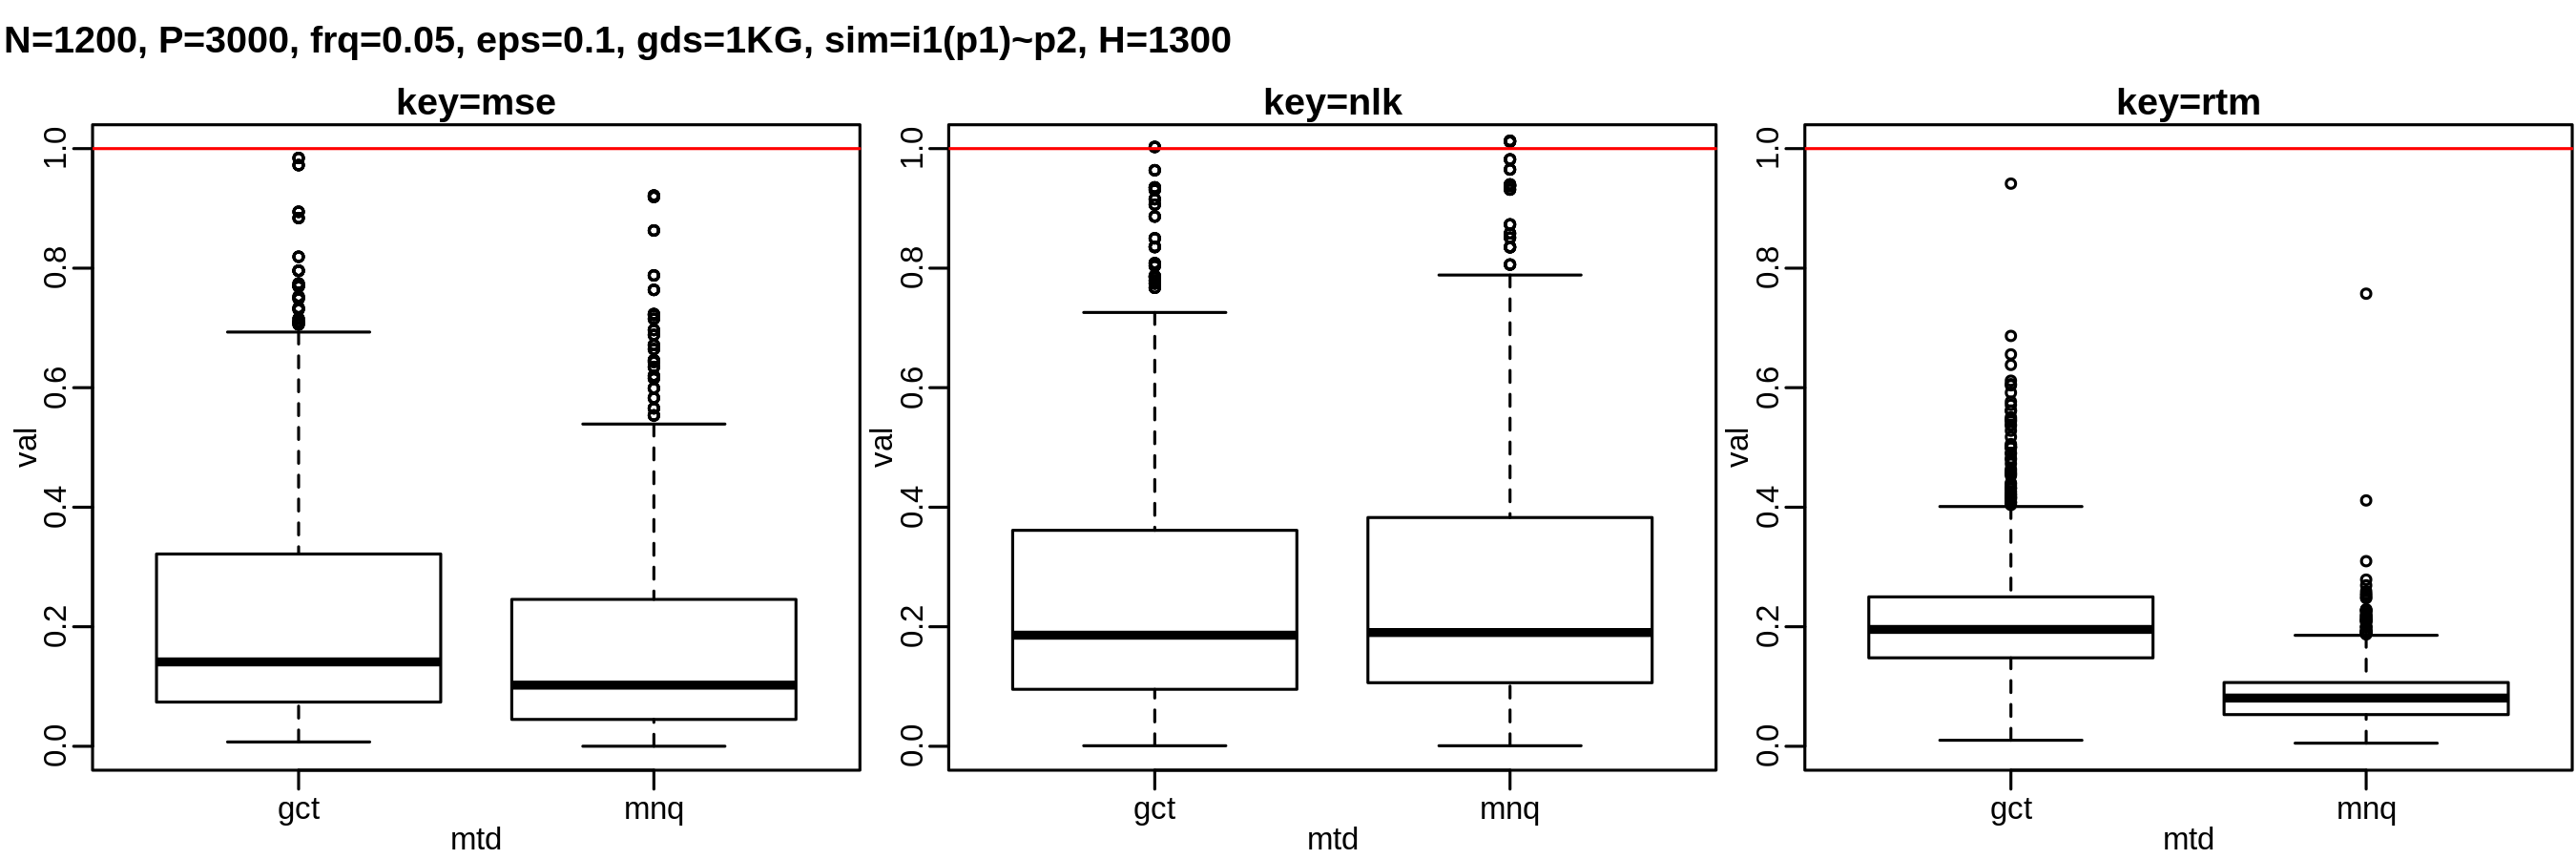
\includegraphics[width=.95\linewidth]{img/1kg_whl_p01}
  \end{figure}
  \textbf{\color{blue}{inner plot: strategies, from left to right:}}
  \begin{itemize}
  \item \textbf{gct:} VCM by GCTA-REML (\textbf{Yang et. al., 2011})
  \item \textbf{mnq:} Improved VCM by MINQUE
  \end{itemize}
\end{frame}
% -------------------------------------------------------------------
\begin{frame}\frametitle{simulation 1: improved VCM versus REML-VCM}
  \textbf{data: $h(\vy)=\text{zscore}[(\va + \one)^2]$} \\
  \begin{figure}
    \centering 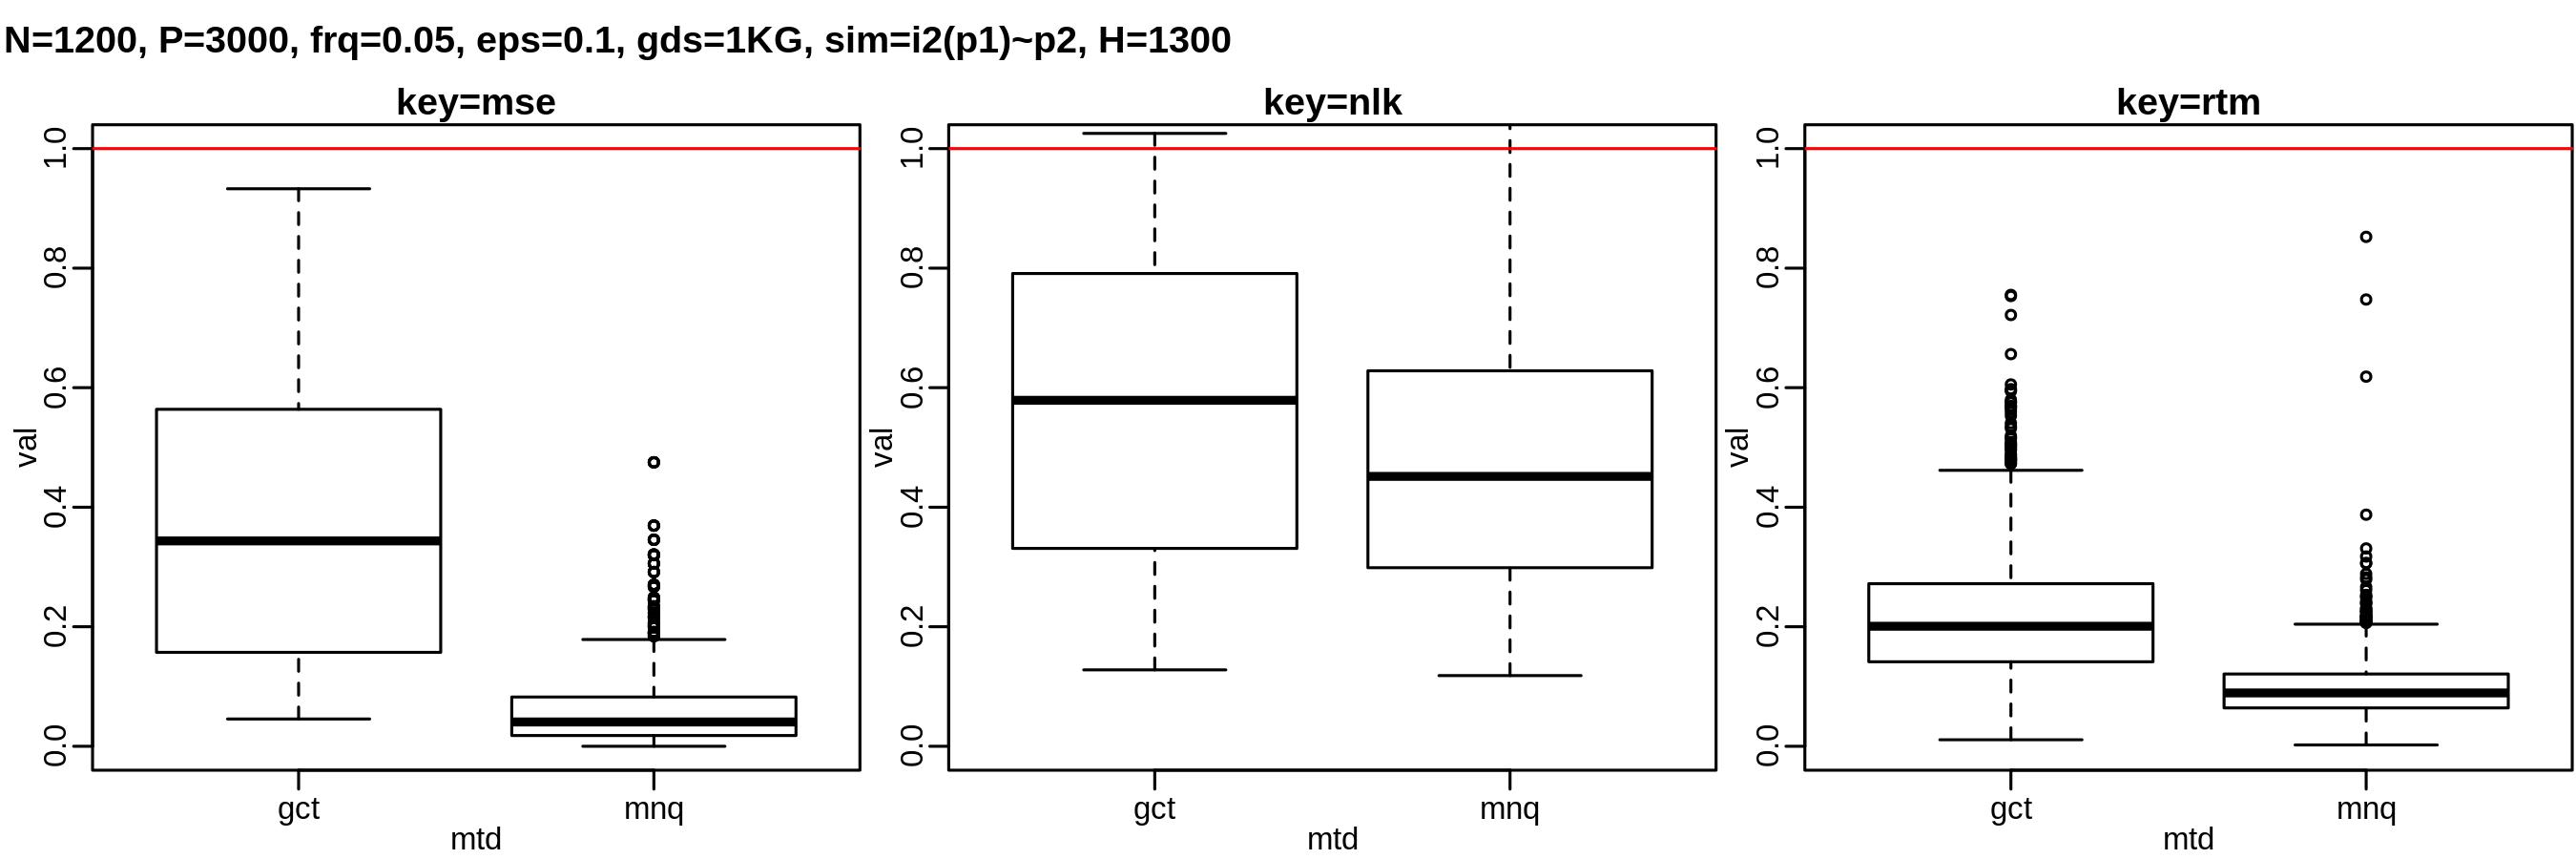
\includegraphics[width=.95\linewidth]{img/1kg_whl_p02}
  \end{figure}
  \textbf{\color{blue}{inner plot: strategies, from left to right:}}
  \begin{itemize}
  \item \textbf{gct:} VCM by GCTA-REML (\textbf{Yang et. al., 2011})
  \item \textbf{mnq:} Improved VCM by MINQUE
  \end{itemize}
\end{frame}
% -------------------------------------------------------------------
\subsection{simulation 2: batched versus whole sample VCM}
\begin{frame}\frametitle{simulation 1: Improved VCM versus REML}
  \textbf{Train on 1200 samples, test on another 1300;} \\
  \textbf{Batch size varied from 100 to 400;} \\
  {\color{blue}\textbf{performance measurement:}}
  \begin{itemize}
  \item \textbf{MSE:} mean square error;
  \item \textbf{NLK:} mean negative log likelihood;
  \item \textbf{RTM:} running time;
  \end{itemize}
  \CB{\textbf{data generation:}}
  \begin{itemize}
  \item \textbf{signals:} $\va \sim \mathcal{N}(\bm{0}, \sigma_0^2\id + \sigma_1^2\mZ\mZ^T)$
  \item \textbf{order 1:} $h(\vy)=\va$;
  \item \textbf{order 2:} $h(\vy)=\text{zscore}[(\va + \one)^2]$.
  \end{itemize}
\end{frame}
% -------------------------------------------------------------------
\begin{frame}\frametitle{simulation 2: batched VCM versus whole sample}
  \textbf{data: $h(\vy)=\va$} \\
  \begin{figure}
    \centering 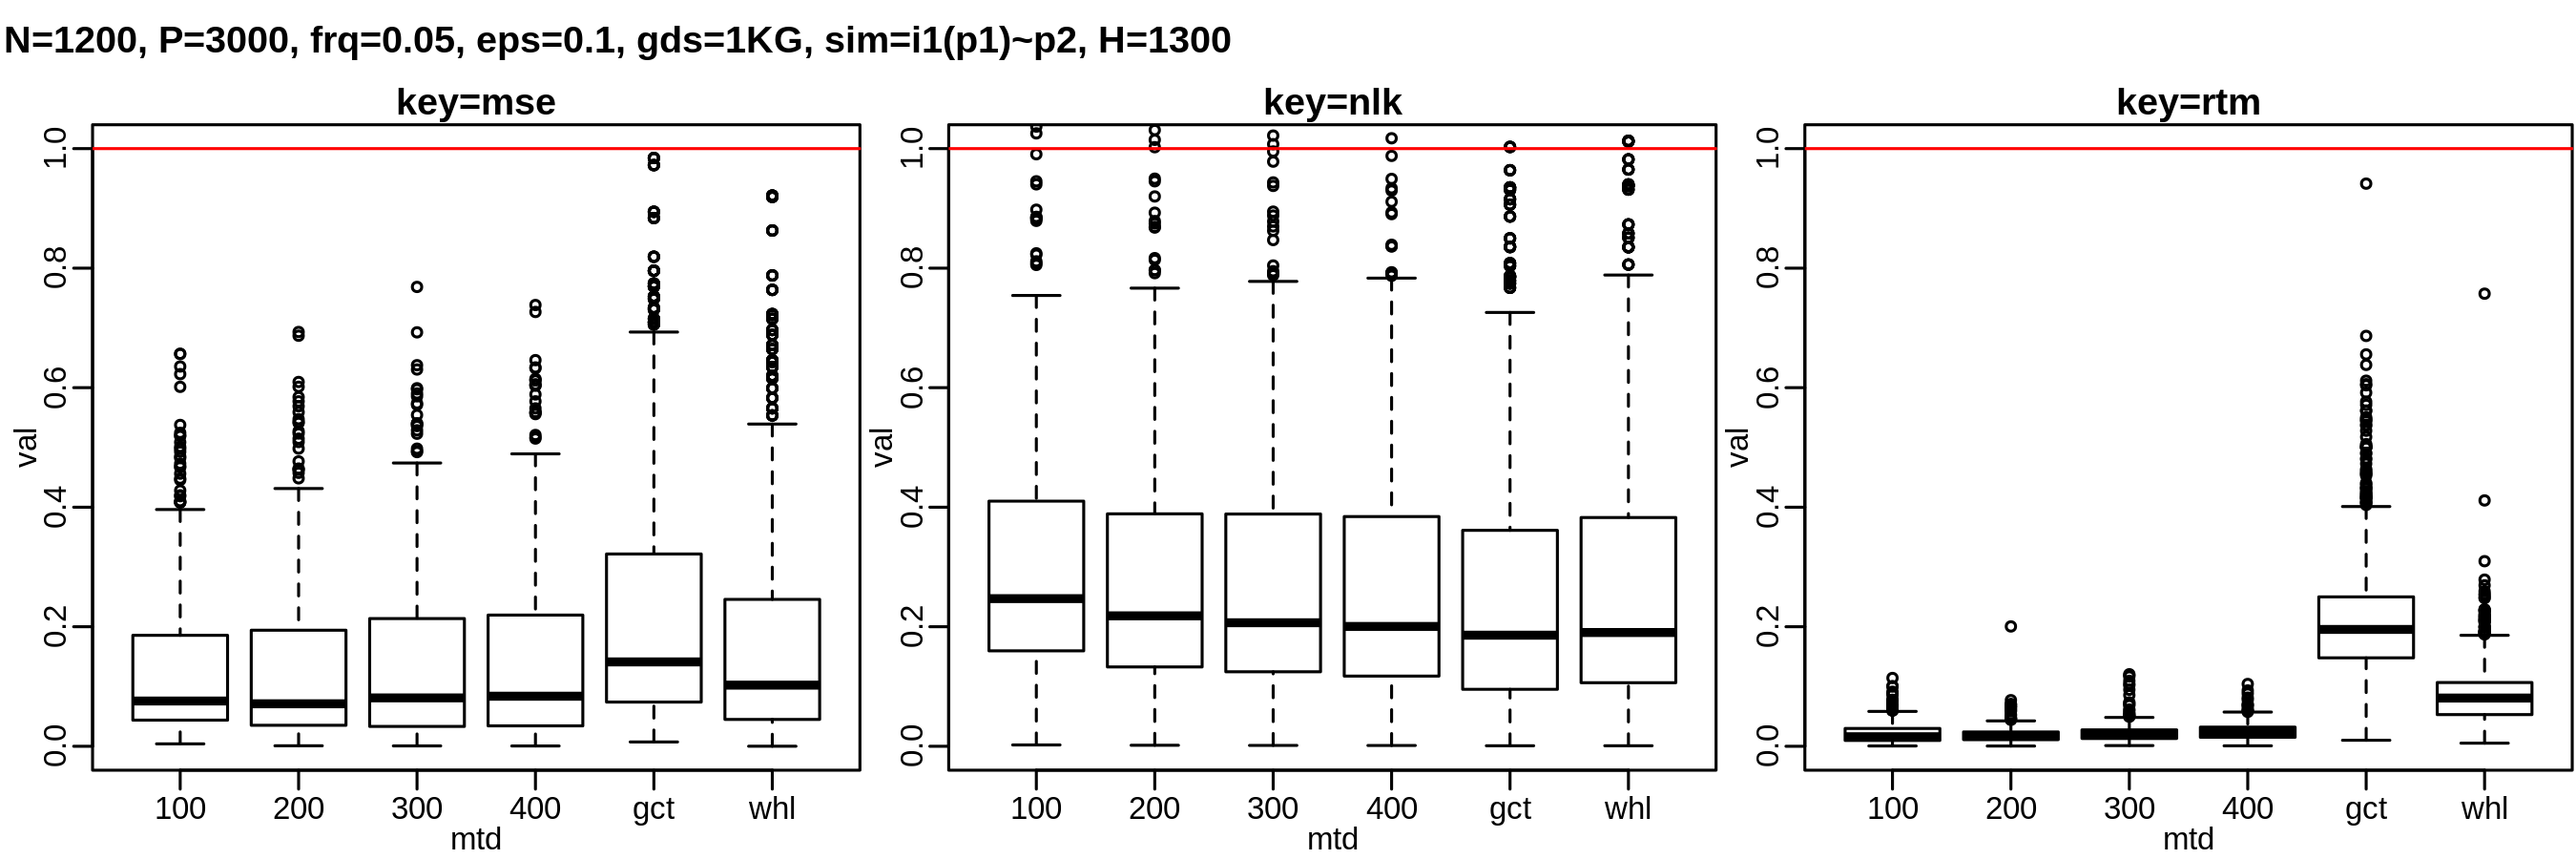
\includegraphics[width=1\linewidth]{img/1kg_bat_p01}
  \end{figure}
  \textbf{\color{blue}{inner plot: strategies, from left to right:}}
  \begin{itemize}
  \item \textbf{gct:} GCTA-REML on the entire sample;
  \item \textbf{100 - 400, whl:} batched and whole sample VCM by MINQUE
  \end{itemize}
\end{frame}
% -------------------------------------------------------------------
\begin{frame}\frametitle{simulation 2: batched VCM versus whole sample}
  \textbf{data: $h(\vy)=\text{zscore}[(\va + \one)^2]$} \\
  \begin{figure}
    \centering 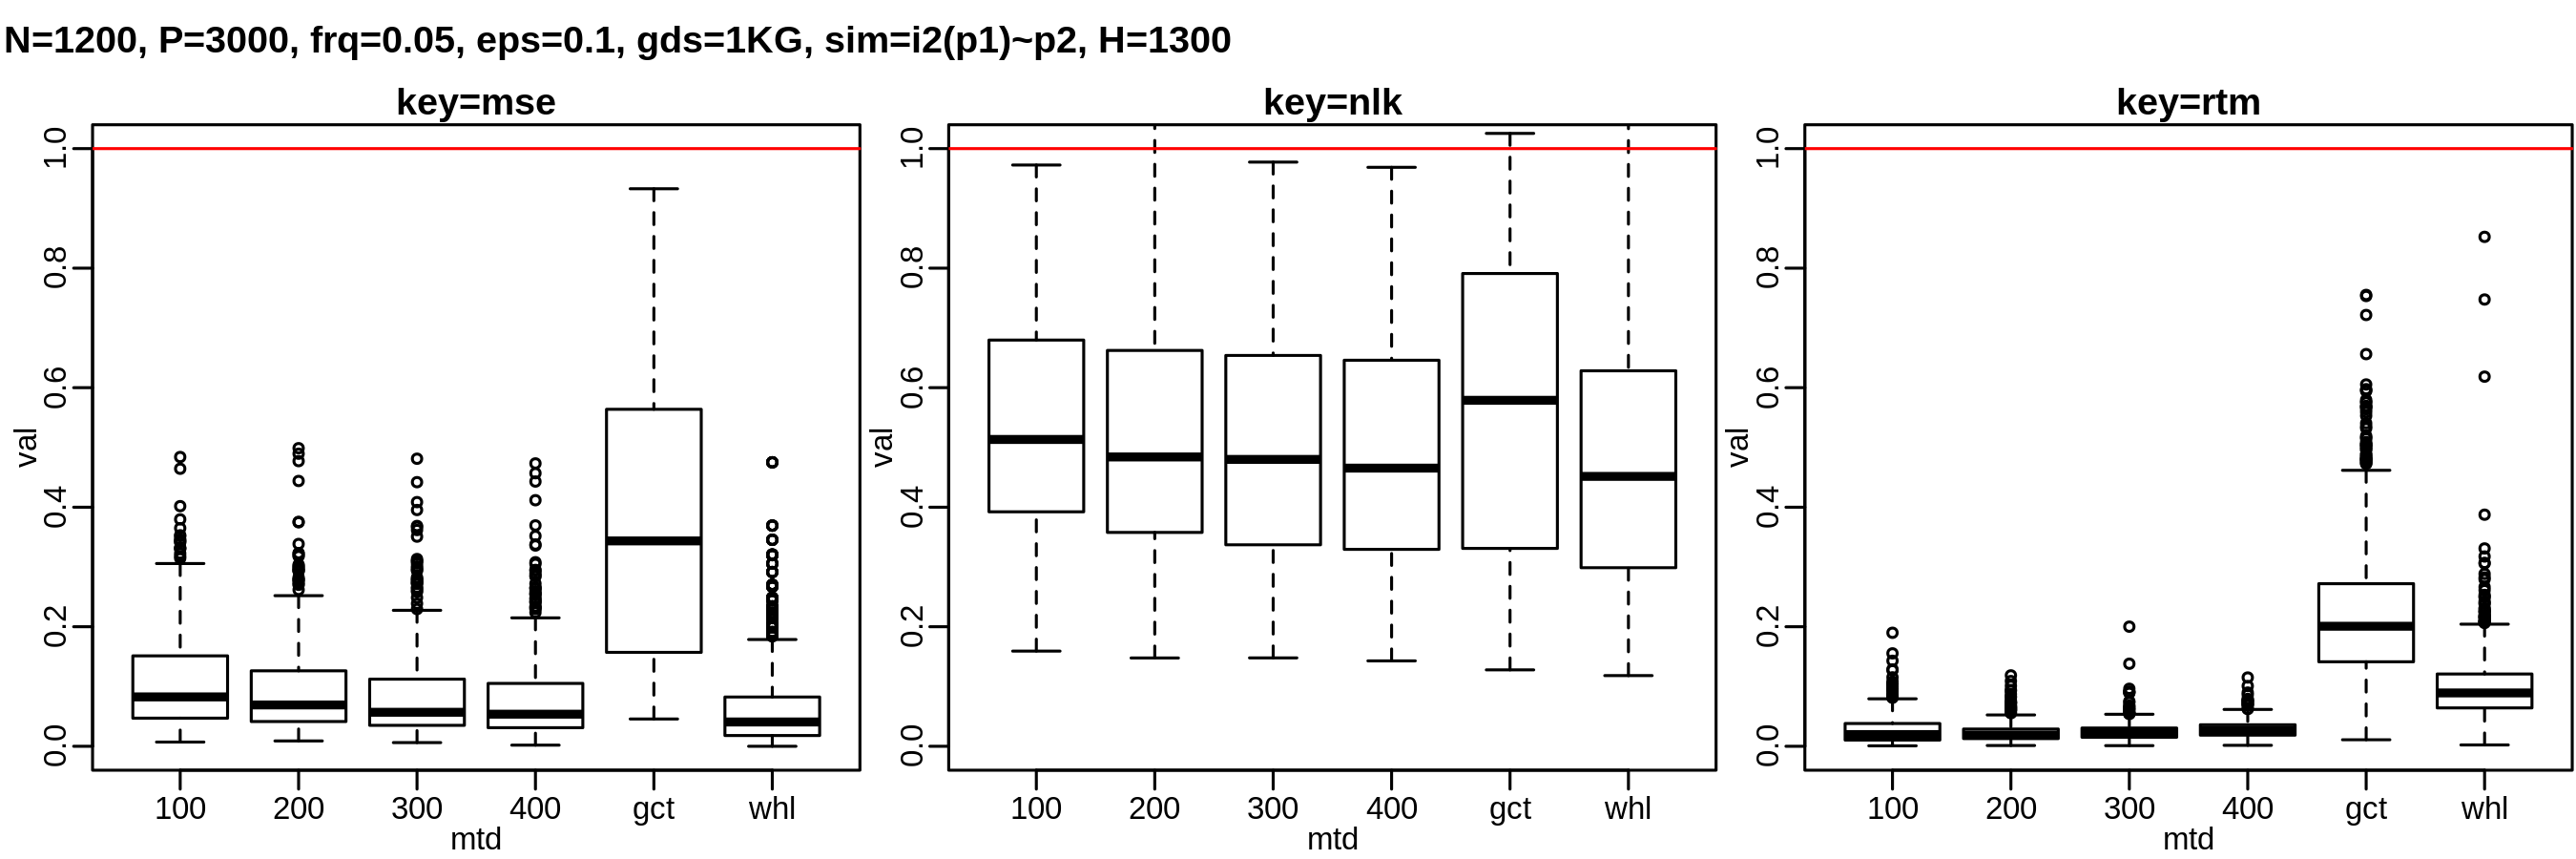
\includegraphics[width=1\linewidth]{img/1kg_bat_p02}
  \end{figure}
  \textbf{\color{blue}{inner plot: strategies, from left to right:}}
  \begin{itemize}
  \item \textbf{gct:} GCTA-REML on the entire sample;
  \item \textbf{100 - 400, whl:} batched and whole sample VCM by MINQUE
  \end{itemize}
\end{frame}
% -------------------------------------------------------------------
\subsection{simulation 3: performance by sample sizes}
\begin{frame}\frametitle{simulation 1: Improved VCM versus REML}
  \textbf{Train on 100 to 1000 samples, test on another 1000;} \\
  {\color{blue}\textbf{performance measurement:}}
  \begin{itemize}
  \item \textbf{MSE:} mean square error;
  \item \textbf{NLK:} mean negative log likelihood;
  \item \textbf{RTM:} running time;
  \end{itemize}
  \CB{\textbf{data generation:}}
  \begin{itemize}
  \item \textbf{signals:} $\va \sim \mathcal{N}(\bm{0}, \sigma_0^2\id + \sigma_1^2\mX\mX^T)$
  \item \textbf{order 2:} $h(\vy)=\text{zscore}[(\va + \one)^2]$.
  \end{itemize}
\end{frame}
% -------------------------------------------------------------------
\begin{frame}\frametitle{simulation 3: performance by sample sizes}
  \textbf{data: $h(\vy)=\text{zscore}[(\va + \one)^2]$} \\
  \begin{figure}
    \centering 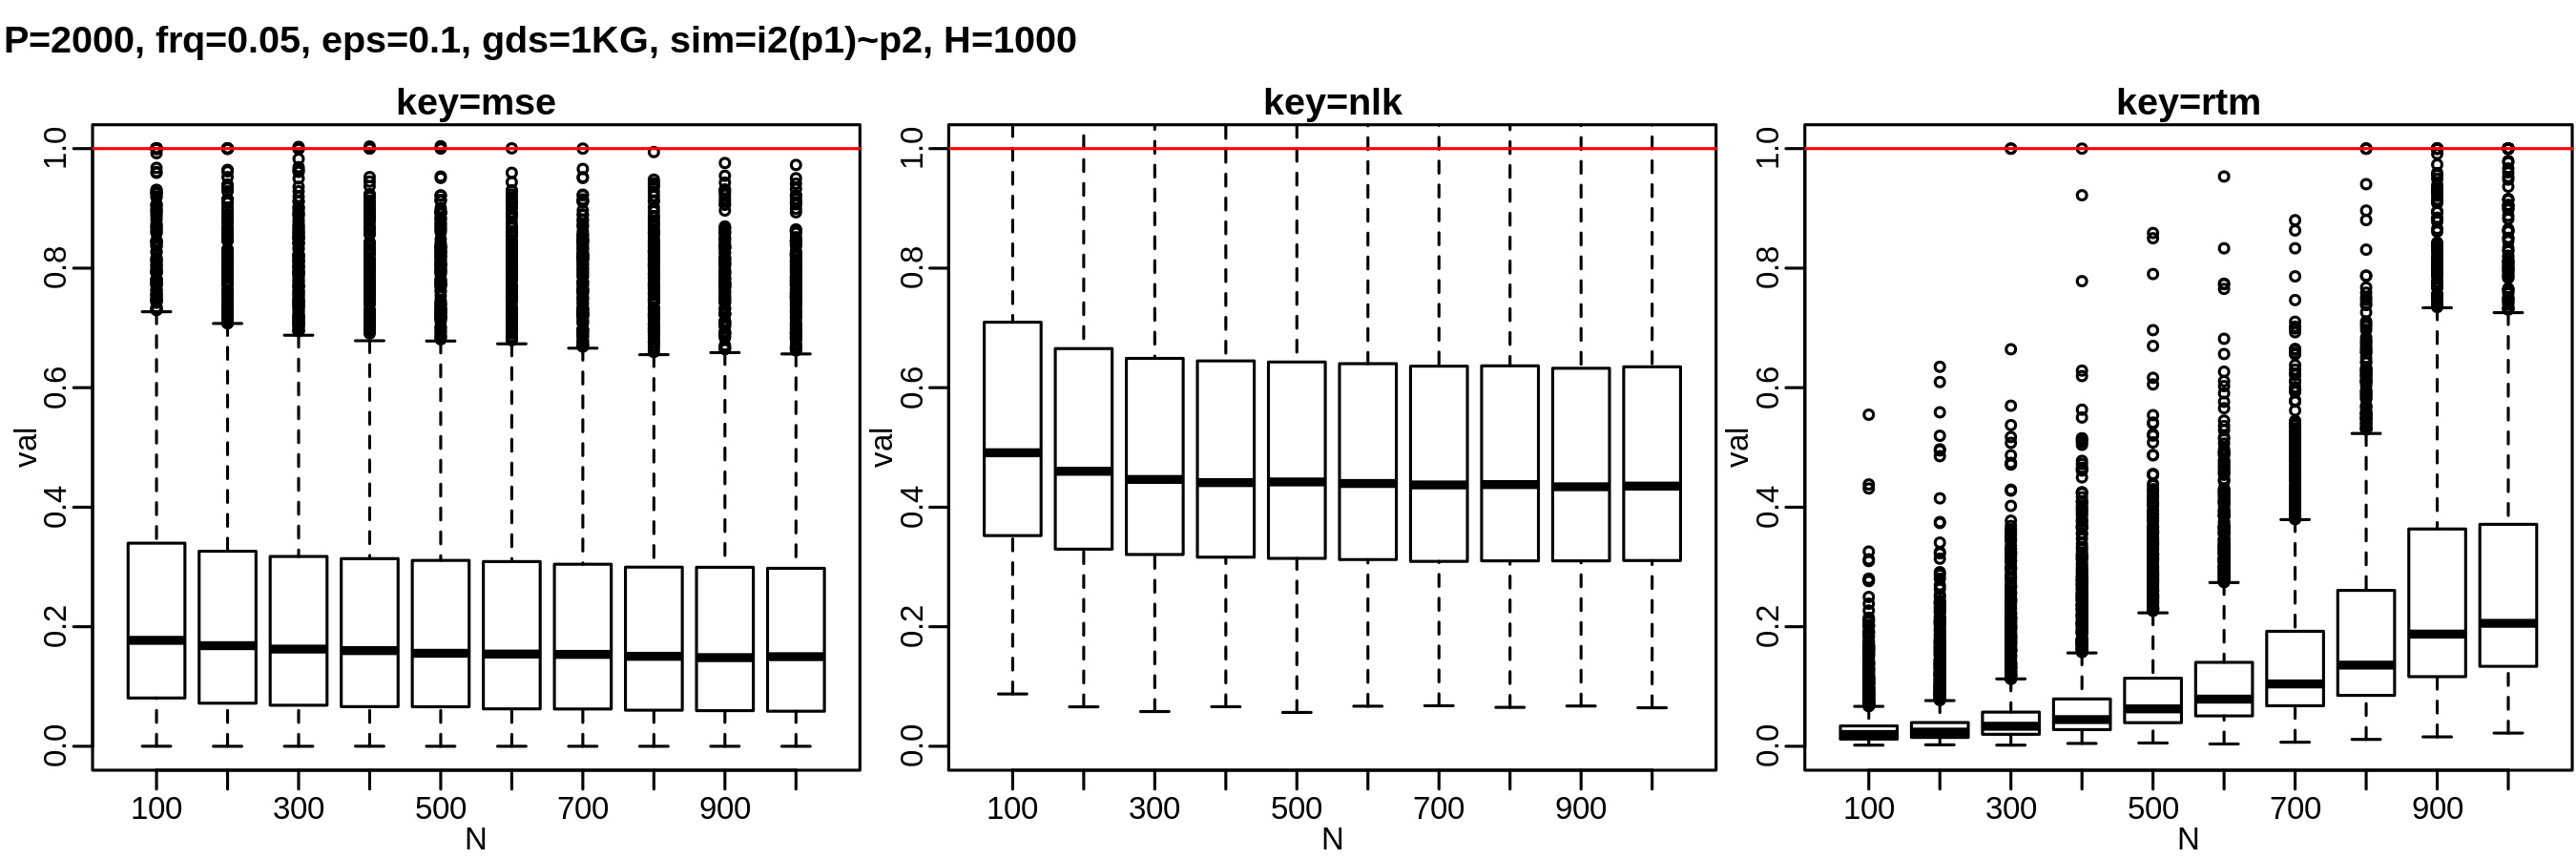
\includegraphics[width=.95\linewidth]{img/1kg_whl_t02}
  \end{figure}
  \textbf{\color{blue}{inner plot: sample sizes}}
\end{frame}
% -------------------------------------------------------------------
% \section{Theoratical Ground}
\begin{frame} <presentation:0> %
  \frametitle{Theoretical Ground} %
  \textbf{How meta-VCM built on incomplete data outperform maga-VCM?} \\
  Let $\ve=[e_1 \dots e_Q]$ be the validation error made by the $Q$
  client models on a unseen random data point, such that
  \begin{itemize}
  \item $\E(e_i) = v$
  \item $\E(e_i e_j) = c$
  \end{itemize}
  The average error made by all $Q$ models is $\frac{1}{k}\sum_i e_i$,
  and
  \begin{align} \label{eq:beg} \E\left[ \left(\frac{1}{k}\sum_i
        e_i\right)^2 \right]
    &= \frac{1}{k^2}\E\left[\sum_i \left(e_i^2 + \sum_{j \ne i}e_ie_j \right)  \right] \\
    &= \frac{1}{k}v + \frac{k-1}{k}c
  \end{align}
\end{frame}
% -------------------------------------------------------------------
\begin{frame} <presentation:0>%
  \frametitle{Theoretical Ground}%
  \textbf{when inter-cohort heterogeneity increases:}
  \begin{itemize}
  \item VCMs become less correlated, $\E(e_i e_j) = c$ goes to 0;
  \item $\E\left[ \left(\frac{1}{k}\sum_i e_i\right)^2 \right]$
    shrinks to $\frac{v}{k}$ -- averaging VCMs benefits;
  \item heterogeneity act as noise for the full, mega-VCM;
  \end{itemize}
  \textbf{when cohort become more homogeneous:}
  \begin{itemize}
  \item VCMs become more correlated, $\E(e_i e_j) = c$ goes to 1;
  \item $\E\left[ \left(\frac{1}{k}\sum_i e_i\right)^2 \right]$
    remains to be $v$ -- averaging VCMs has no effect;
  \item the whole data is less noisy to the full, mega-VCM;
  \end{itemize}
  The model averaging (\ref{eq:beg}) is called ``bootstrap aggregating
  (bagging)'', developed by (Breiman, 1994, et. al.).
\end{frame}
% -------------------------------------------------------------------
\section{Summary}
\begin{frame} %
  \frametitle{Summary} %
  \textbf{The combination of}
  \begin{itemize}
  \item Batched training,
  \item kernel deepening,
  \item and MINQUE solver
  \end{itemize}
  achieved better balance of capacity and cost of for VCM. \\
  \textbf{Factors that diminish the advantages of deep kernel:}
  \begin{itemize}
  \item a growing number of variants;
  \item enlarged true white noise;
  \item reduced size of true variance components.
  \end{itemize}
  \textbf{About UK Biobank's genomic data}
  \begin{itemize}
  \item MINQUE solution maybe fail in terms of log likelihood.
  \end{itemize}
\end{frame}
% -------------------------------------------------------------------
\begin{frame} %
  \frametitle{Contact} %
  Xiaoran Tong \\
  Department of Epidemiology \& Biostatistics \\
  Michigan State University
  \begin{itemize}
  \item email: tongxia1@msu.edu
  \item phone: (1)517-220-1229
  \end{itemize}
\end{frame}
\end{document}
